\documentclass{beamer}
\hypersetup{colorlinks=true}
\graphicspath{{./images/}}
\usefonttheme{professionalfonts}
\usefonttheme{serif}
\usepackage{fontspec}
\setmainfont{Roboto Slab}
\usepackage{multicol}

\title{Superfast modeling in PlantUML}
\subtitle{Workshop PlantUML for creating UML diagrams}
\author{Sander van Geloven}
\institute{Hellebaard}
\date{May 11, 2019}
\keywords{PlantUML, UML, modeling, modelling, workshop}

\begin{document}

\begin{frame}
\titlepage
\end{frame}

\section*{Outline}
\begin{frame}
\tableofcontents
\end{frame}



\begin{frame}{Introduction}
Sander van Geloven
\\\mbox{}
\begin{itemize}
\item information analyst / ICT architect
\\\mbox{}
\item self-employed at \href{http://hellebaard.nl}{hellebaard.nl}
\\\mbox{}
\item curriculum vitae at \href{https://linkedin.com/in/svgeloven}{linkedin.com/in/svgeloven}
\\\mbox{}
\item writing tools for spelling and grammar 
\\\mbox{}
\begin{itemize}
\item Dutch spelling and grammar \href{http://opentaal.org}{opentaal.org}
\item Dutch word list \href{http://woordenlijst.org}{woordenlijst.org}
\item spell checker \href{https://nuspell.github.io}{nuspell.github.io}
\end{itemize}
\end{itemize}
\end{frame}



\section{Unified Modeling Language (UML)}

\begin{frame}{Unified Modeling Language (UML) — What is it?}
\begin{columns}
\begin{column}{.6\textwidth}
\begin{itemize}
\item \alert{modeling language for visualizing system design}
\\\mbox{}
\item designed in 1994 – 1996 by
\begin{itemize}
\item Grady Booch (1955)
\item Ivar Jacobson (1939)
\item James Rumbaugh (1947)
\end{itemize}
\mbox{}
\item \alert{diagrams to represent structural and behavior information}, including interaction aspects
\\\mbox{}
\item version 2.5.1, 5 December 2017, 800 pages, \href{http://uml.org}{uml.org}
\end{itemize}
\end{column}
\begin{column}{.4\textwidth}
\begin{figure}
\def\centering\svgwidth{\columnwidth}
\resizebox{\columnwidth}{!}{\input{images/logo-uml.pdf_tex}}
\end{figure}
\end{column}
\end{columns}
\end{frame}

\begin{frame}{UML — No more flow charts on a back of a coaster}
\begin{figure}
\centering
\resizebox{!}{.75\textheight}{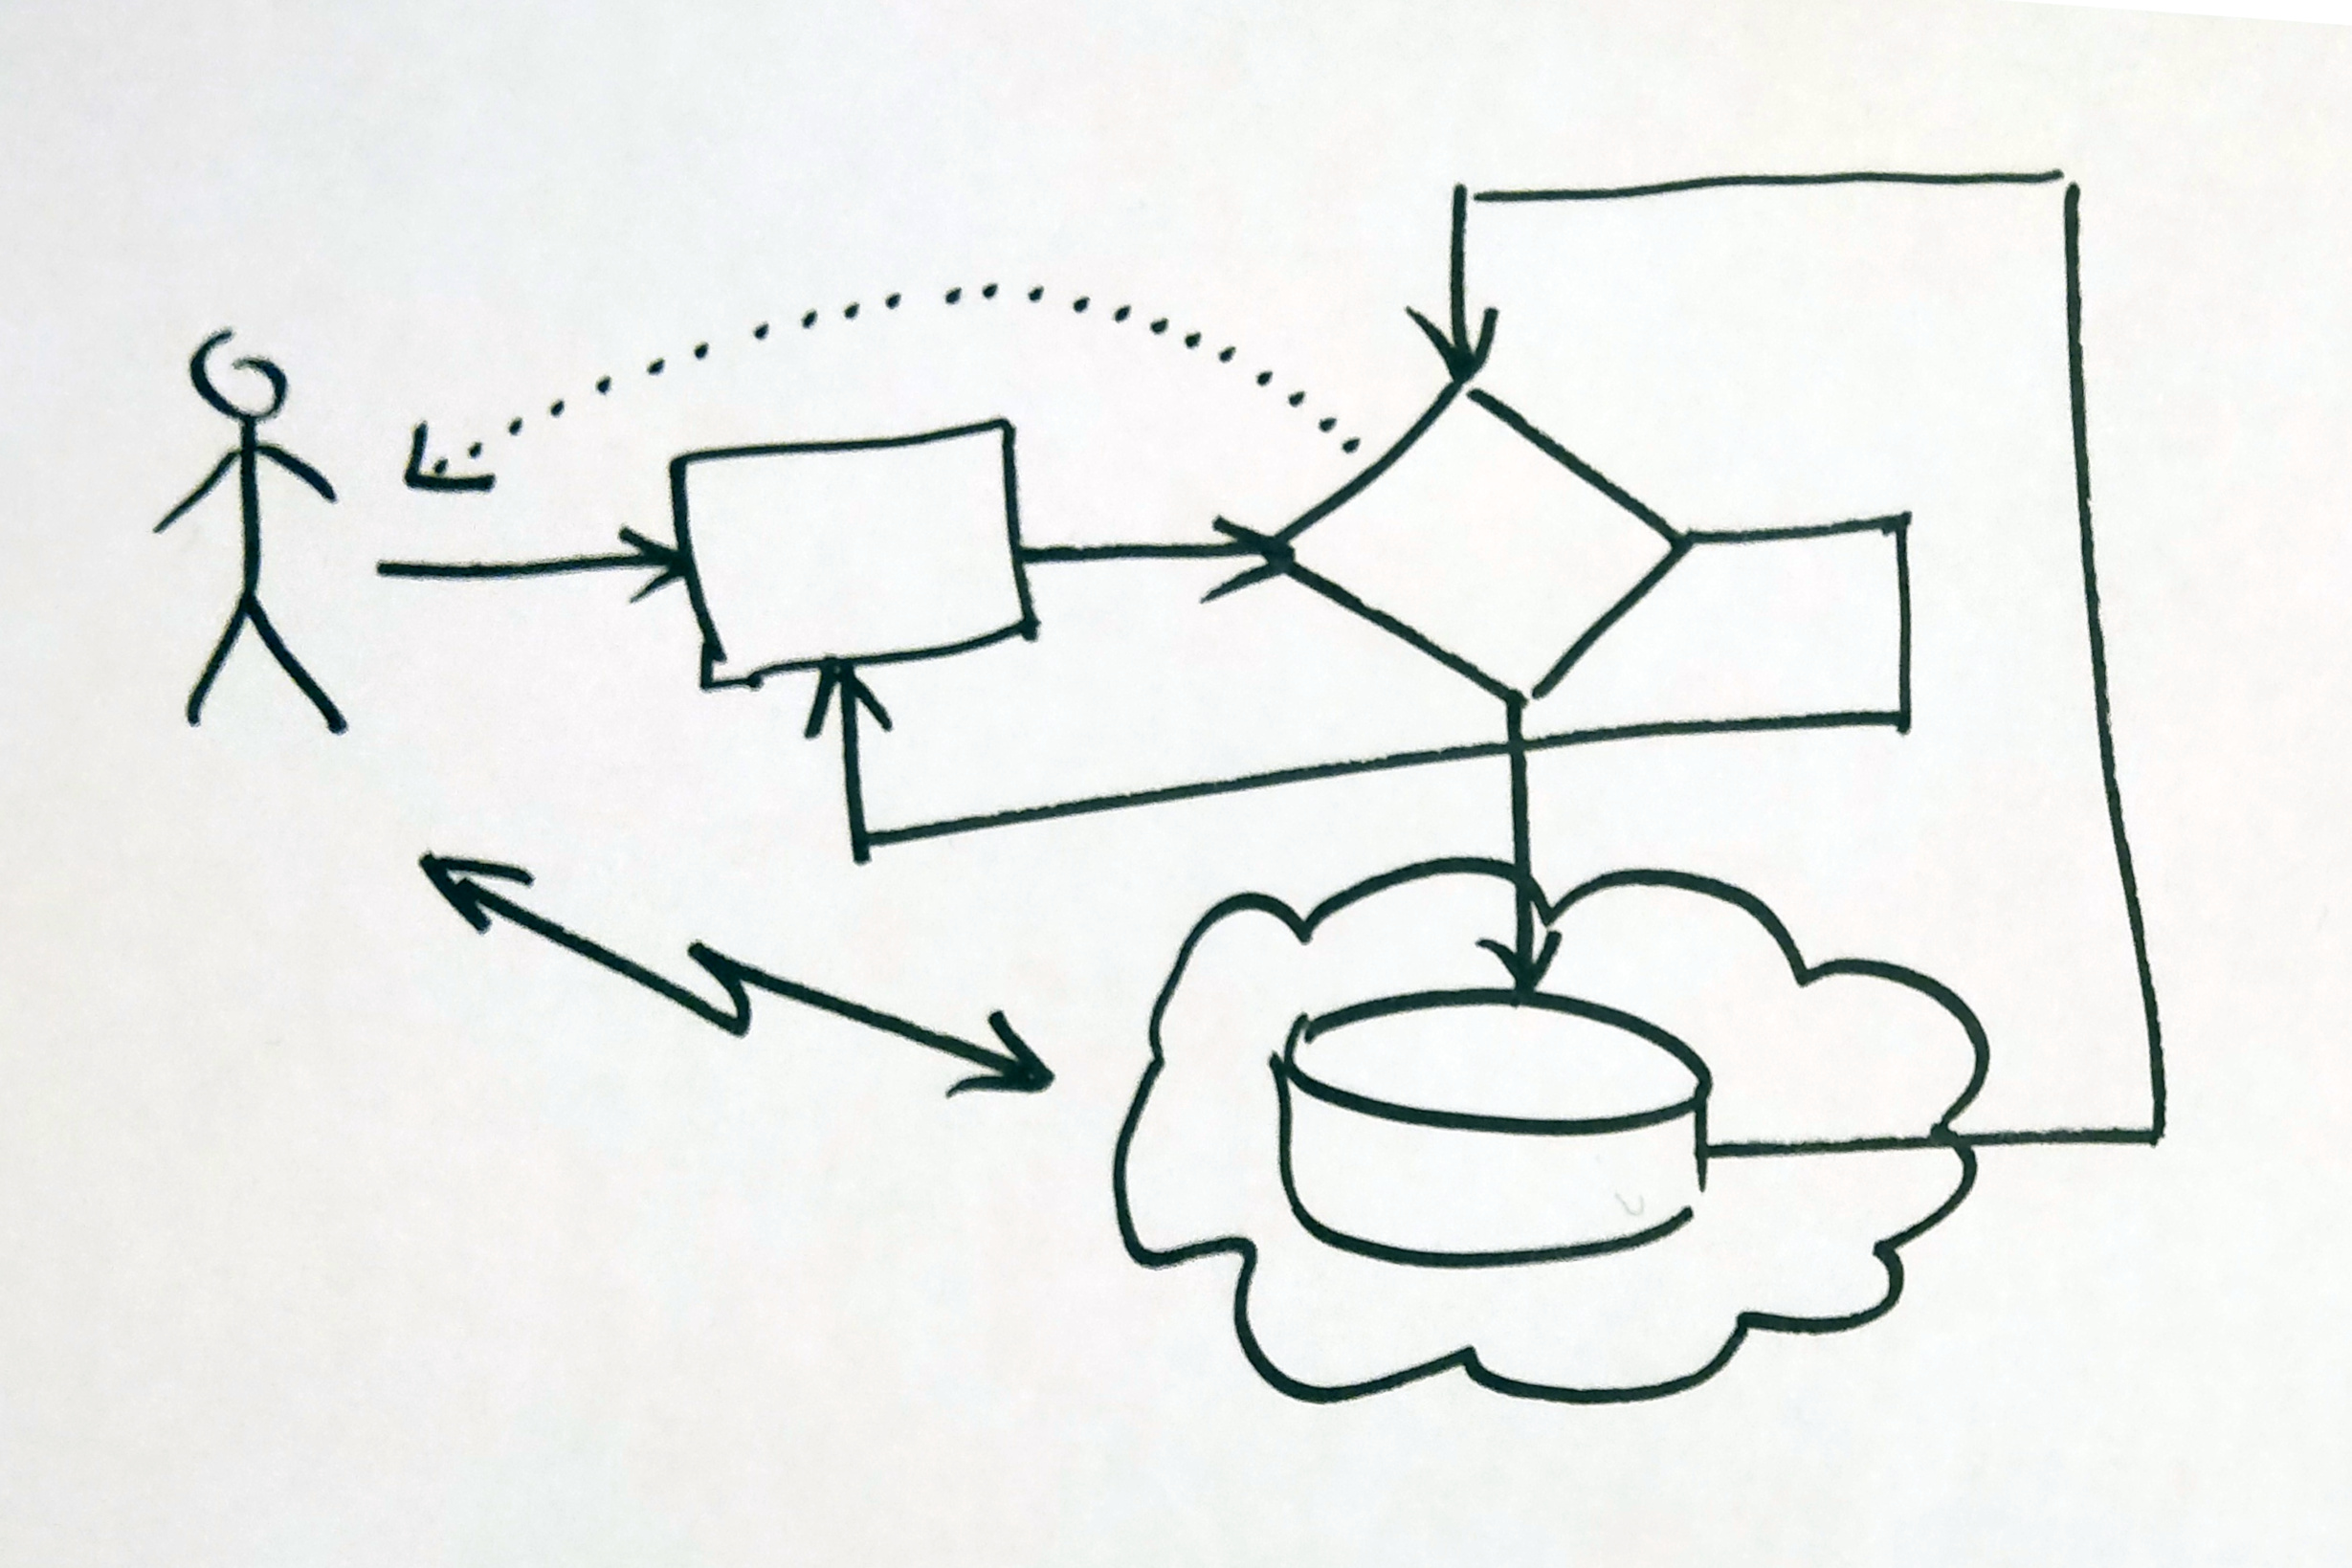
\includegraphics{images/coaster.jpg}}
\end{figure}
\end{frame}

\begin{frame}{UML — Common problems}
Common problems with visual editors for UML diagrams:
\\\mbox{}
\begin{enumerate}
\item wasting time positioning and repositioning elements
\\\mbox{}
\item wasting time untangling intersecting lines
\\\mbox{}
\item wasting time setting (partially working) grid snap
\\\mbox{}
\item wasting time applying font and font alignment
\\\mbox{}
\item wasting time and risking RSI while micro-aligning
\end{enumerate}
\end{frame}



\section{PlantUML}

\begin{frame}{PlantUML — What is it?}
\begin{columns}
\begin{column}{.6\textwidth}
\begin{itemize}
\item \alert{FOSS tool to create UML diagrams from plain text}
\\\mbox{}
\item developed 2009 – 2019 by Arnaud Roques
\\\mbox{}
\item GPLv3 but also LGPL, GPLv2, Apache License, Eclipse Public License and MIT License
\\\mbox{}
\item version 1.2019.5, 23 April 2019, \alert{17 types of diagrams}, \alert{12 output file formats}, \href{http://plantuml.com}{plantuml.com}
\end{itemize}
\end{column}
\begin{column}{.4\textwidth}
\begin{figure}
\def\centering\svgwidth{\columnwidth}
\resizebox{\columnwidth}{!}{\input{images/logo-plantuml.pdf_tex}}
\end{figure}
\end{column}
\end{columns}
\end{frame}

\begin{frame}{PlantUML — How it works}
PlantUML:
\\\mbox{}
\begin{itemize}
\item uses the FOSS graph rendering \alert{Graphviz}, \href{https://graphviz.org}{graphviz.org}\\
for example \texttt{a -> b} creates\\
\begin{figure}
\centering
\resizebox{!}{.1\textheight}{\includegraphics{images/a.png}}
\end{figure}
\item has text file (\texttt{.puml} or \texttt{.pu}) as input
\\\mbox{}
\item generates diagram in output file or in a GUI
\\\mbox{}
\item uses \alert{convention over configuration}, yet is \alert{highly configurable}
\end{itemize}
\end{frame}

\begin{frame}{PlantUML ­— Supported UML diagrams}
UML behavior diagrams:
\begin{enumerate}
\item activity diagram
\item sequence diagram
\item timing diagram
\item state diagram
\item usecase diagram
\end{enumerate}
\mbox{}\\
UML structure diagrams:
\begin{enumerate}\setcounter{enumi}{5}
\item class diagram
\item deployment diagram
\item component diagram
\item object diagram
\end{enumerate}
\end{frame}

\begin{frame}{PlantUML — Supported non-UML diagrams}
Supported non-UML diagrams:
\begin{enumerate}
\item wireframe graphical interface
\item Archimate diagram
\item Specification and Description Language (SDL) diagram
\item Ditaa diagram
\item Gannt diagram
\item MindMap diagram
\item work breakdown structure diagram
\item mathematic with AsciiMath or JLaTeXMath notation
\end{enumerate}
\mbox{}\\
PlantUML is used by \alert{many} wikis, forums, text editors, IDE, programming languages and documentation generators.
\end{frame}

\begin{frame}{PlantUML — Supported output formats}
\begin{enumerate}
\item \texttt{gui} - Graphical User-Interface (your screen)
\item \texttt{png} - Portable Network Graphics (default)
\item \texttt{svg} - \alert{Scalable} Vector Graphics
\item \texttt{eps} - Encapsulated PostScript
\item \texttt{pdf} - Portable Document Format
\item \texttt{vdx} - Virtual Document eXchange
\item \texttt{xmi} - XML Metadata Interchange (class diagram)
\item \texttt{txt} - ASCII art
\item \texttt{utxt} - ASCII art using Unicode characters
\item \texttt{html} - Hypertext Markup Language (class diagram)
\item \texttt{scxml} - State Chart XML (state diagram)
\item \texttt{latex} - LaTeX/Tikz format
\item \texttt{latex:nopreamble} - LaTeX/Tikz format w/o preamble
\end{enumerate}
\end{frame}



\section{1~~~Usecase Diagram}

\begin{frame}[fragile]{1~~~Usecase Diagram — Simple example}
\begin{columns}
\begin{column}{.6\textwidth}
overview of \alert{users} in relation to functional requirements in \alert{usecases}
\begin{verbatim}
left to right direction

User <|-right- Admin : derives

User --> (Usecase 1)
Admin --> (Usecase 2)

(Usecase 3) .left.> (Usecase 1)
 : extends
\end{verbatim}
Note that the arrow directions are rotated 90° clockwise.
\end{column}
\begin{column}{.4\textwidth}
\begin{figure}
\def\centering\svgwidth{\columnwidth}
\resizebox{!}{.5\textheight}{\input{images/usecase-diagram.pdf_tex}}
\end{figure}
\end{column}
\end{columns}
\end{frame}

\begin{frame}{1~~~Usecase Diagram — Exercise}
\begin{columns}
\begin{column}{.35\textwidth}
Exercise 1/5:
\\\mbox{}\\
Make a minimal and optimized usecase diagram in PlantUML that describes the the roles of customers and staff eating and working at a restaurant.
\end{column}
\begin{column}{.65\textwidth}
\begin{figure}
\centering
\resizebox{!}{.75\textheight}{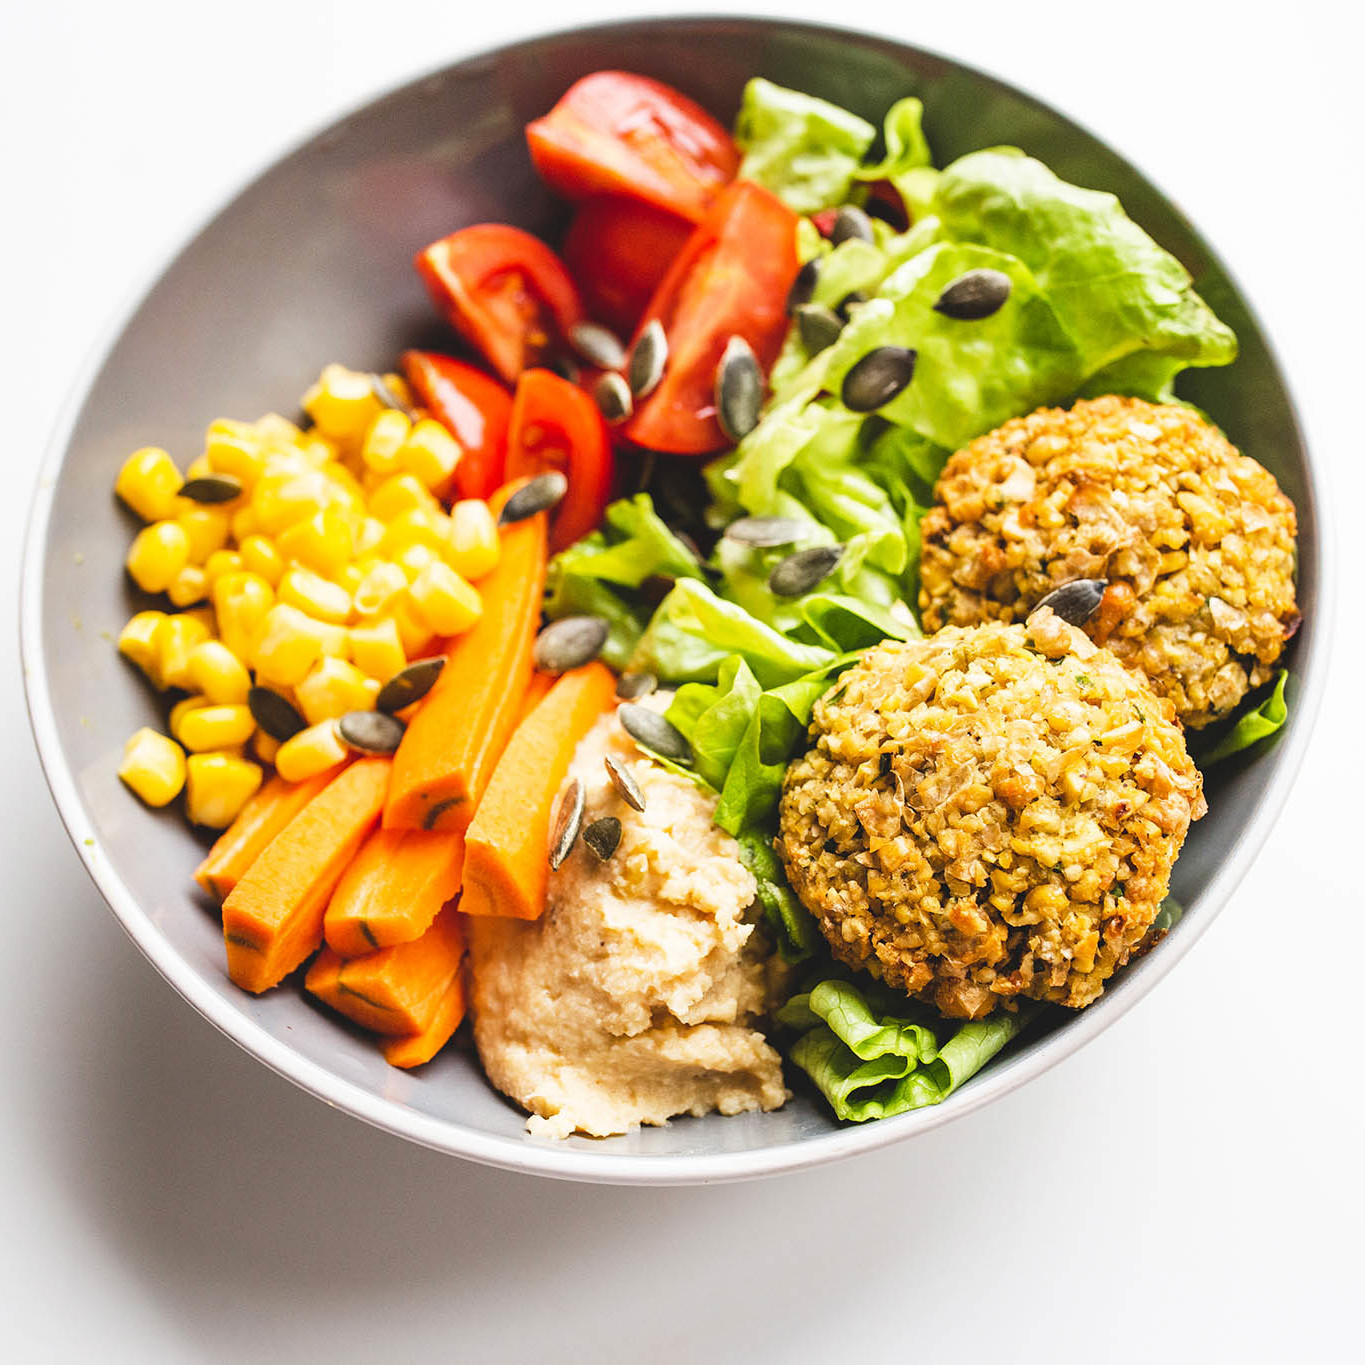
\includegraphics{images/dish.jpg}}
\end{figure}
\end{column}
\end{columns}
\end{frame}

\begin{frame}{1~~~Usecase Diagram — Restaurant}
A customer \alert{may}:
\begin{itemize}
\item order
\item eat
\item pay
\end{itemize}
\mbox{}\\
Staff \alert{may}:
\begin{itemize}
\item serve
\item cook
\item charge
\end{itemize}
\mbox{}\\
All staff \alert{can also use} the restaurant in the \alert{role} of a customer.
\end{frame}

\begin{frame}[fragile]{1~~~Usecase Diagram — Restaurant}
\begin{verbatim}
left to right direction

Customer --> (order)
Customer --> (eat)
Customer --> (pay)
Staff --> (serve)
Staff --> (cook)
Staff --> (charge)

Customer <|-right- Staff
\end{verbatim}
\end{frame}

\begin{frame}{1~~~Usecase Diagram — Restaurant}
\begin{figure}
\def\centering\svgwidth{\textwidth}
\resizebox{!}{.7\textheight}{\input{images/usecase-diagram-minimal.pdf_tex}}
\end{figure}
\end{frame}

\begin{frame}[fragile]{1~~~Usecase Diagram — Restaurant}
\begin{verbatim}
skinparam TitleFontStyle Bold
skinparam ArrowColor Black
skinparam ActorBorderColor Black
skinparam UsecaseBorderColor Black
skinparam ActorBackgroundColor White
skinparam UsecaseBackgroundColor White
Title Usecase Diagram — Restaurant

left to right direction

Customer --> (order)
Customer --> (eat)
Customer --> (pay)
\end{verbatim}
\end{frame}

\begin{frame}{1~~~Usecase Diagram — Restaurant}
\begin{figure}
\def\centering\svgwidth{\textwidth}
\resizebox{.8\textwidth}{!}{\input{images/usecase-diagram-extended.pdf_tex}}
\end{figure} 
\end{frame}



\section{2~~~Activity Diagram}

\begin{frame}[fragile]{2~~~Activity Diagram — Simple example}
\begin{columns}
\begin{column}{.5\textwidth}
\alert{activities} in \alert{sequence}, \alert{selection}, \alert{iteration} and \alert{parallel}
{\scriptsize\begin{verbatim}
start
:activity 1;
if (condition A?) then (yes)
    :activity 2;
else (no)
    :activity 3;
endif
while (condition B?) is (yes)
    :activity 4;
endwhile (no)
fork
    :activity 5;
fork again
    :activity 6;
end fork
stop
\end{verbatim}}
\end{column}
\begin{column}{.5\textwidth}
\begin{figure}
\def\centering\svgwidth{\columnwidth}
\resizebox{!}{.65\textheight}{\input{images/activity-diagram.pdf_tex}}
\end{figure}
\end{column}
\end{columns}
\end{frame}

\begin{frame}{2~~~Activity Diagram — Exercise}
\begin{columns}
\begin{column}{.35\textwidth}
Exercise 2/5:
\\\mbox{}\\
Make a minimal and optimized activity diagram in PlantUML of making a pot of tea when all items needed are withing reach.
\end{column}
\begin{column}{.65\textwidth}
\begin{figure}
\centering
\resizebox{!}{.75\textheight}{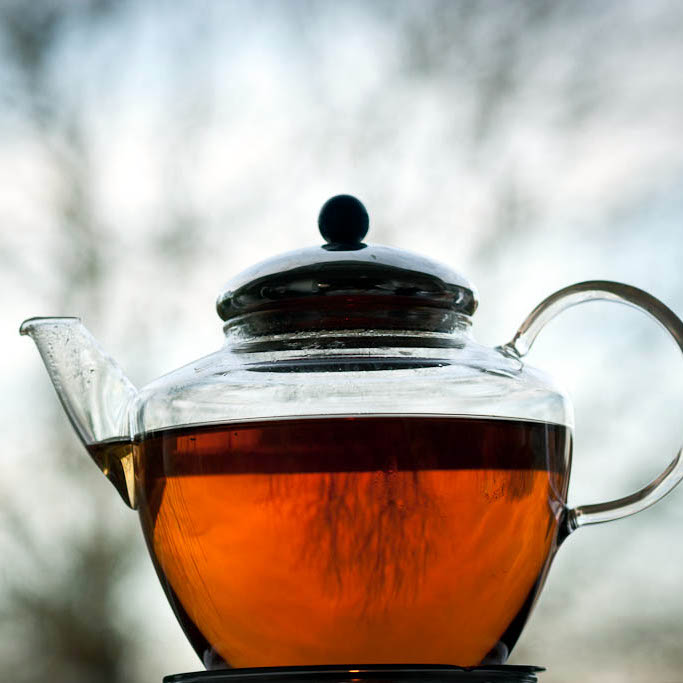
\includegraphics{images/teapot.jpg}}
\end{figure}
\end{column}
\end{columns}
\end{frame}

\begin{frame}{2~~~Activity Diagram — Making tea}
Required \alert{activities}:
\begin{itemize}
\item choose teabag
\item put teabag in teapot
\item switch kettle on
\item fill kettle with water
\item kettle switches heater off
\item poor boiled water from kettle in teapot
\item kettle heats water
\end{itemize}
\mbox{}\\
Required \alert{conditions}:
\begin{itemize}
\item water in kettle is boiling?
\end{itemize}
\end{frame}

\begin{frame}[fragile]{2~~~Activity Diagram — Making tea}
\begin{verbatim}
start
:fill kettle with water;
:switch kettle on;
fork
    while (water in kettle is boiling?) is (no)
        :kettle heats water;
    endwhile (yes)
    :kettle switches heater off;
fork again
    :choose teabag;
    :put teabag in teapot;
end fork
:poor boiled water from kettle in teapot;
stop
\end{verbatim}
\end{frame}

\begin{frame}{2~~~Activity Diagram — Making tea}
\begin{figure}
\def\centering\svgwidth{\textwidth}
\resizebox{!}{.7\textheight}{\input{images/activity-diagram-minimal.pdf_tex}}
\end{figure}
\end{frame}

\begin{frame}[fragile]{2~~~Activity Diagram — Making tea}
\begin{verbatim}
skinparam TitleFontStyle Bold
skinparam ArrowColor Black
skinparam ActivityBorderColor Black
skinparam NoteBorderColor Black
skinparam ActivityBackgroundColor White
skinparam NoteBackgroundColor White
Title Activity Diagram — Making tea

start
:fill kettle with water;
floating note right: use tap water
:switch kettle on;
note right
    <b>after</b> kettle
    is placed back
end note
\end{verbatim}
\end{frame}

\begin{frame}{2~~~Activity Diagram — UML diagrams}
\begin{figure}
\def\centering\svgwidth{\textwidth}
\resizebox{!}{.5\textheight}{\input{images/activity-diagram-extended.pdf_tex}}
\end{figure} 
\end{frame}



\section{3~~~State Diagram}

\begin{frame}[fragile]{3~~~State Diagram — Simple example}
\begin{columns}
\begin{column}{.5\textwidth}
behavioral \alert{state machine} with \alert{events} that trigger \alert{state} transitions
\begin{verbatim}
[*] -down-> StateA
StateA --> StateA : Event 1
StateA -down-> StateB : Event 2
StateB -up-> StateA : Event 3
StateB -down-> [*] : Event 4
\end{verbatim}
Note the \texttt{down} and \texttt{up} arrow directions and that the initial transition has no event.
\end{column}
\begin{column}{.5\textwidth}
\begin{figure}
\def\centering\svgwidth{\columnwidth}
\resizebox{!}{.8\textheight}{\input{images/state-diagram.pdf_tex}}
\end{figure}
\end{column}
\end{columns}
\end{frame}

\begin{frame}{3~~~State Diagram — Exercise}
\begin{columns}
\begin{column}{.35\textwidth}
Exercise 3/5:
\\\mbox{}\\
Make a minimal and optimized state diagram in PlantUML that describes the states and events of a swimming pool locker under normal circumstances.
\end{column}
\begin{column}{.65\textwidth}
\begin{figure}
\centering
\resizebox{!}{.75\textheight}{\includegraphics{images/locker.jpg}}
\end{figure}
\end{column}
\end{columns}
\end{frame}

\begin{frame}{3~~~State Diagram — Swimming pool locker}
Possible \alert{events}:
\\\mbox{}
\begin{itemize}
\item open or close door
\\\mbox{}\\
\item insert coin
\\\mbox{}\\
\item insert or retract key
\\\mbox{}\\
\item turn key clockwise or counterclockwise
\end{itemize}
\end{frame}

\begin{frame}{3~~~State Diagram — Swimming pool locker}
Possible aspects of \alert{states}:
\\\mbox{}
\begin{itemize}
\item door is open, closed or locked
\\\mbox{}\\
\item coin is inserted or not
\\\mbox{}\\
\item key is inserted, turned or retracted
\end{itemize}
\end{frame}

\begin{frame}[fragile]{3~~~State Diagram — Swimming pool locker}
\begin{verbatim}
[*] -right-> Open
Open -right-> OpenCoinIn : insertCoin

OpenCoinIn -down-> ClosedCoinIn : closeDoor
ClosedCoinIn -up-> OpenCoinIn : openDoor

ClosedCoinIn -down-> LockedKeyTurned : turnKeyCCW
LockedKeyTurned -left-> Locked : retractKey
Locked -right-> LockedKeyTurned : insertKey
LockedKeyTurned -left-> Closed : turnKeyCW

Closed -up-> Open : openDoor
Open -down-> Closed : closeDoor
\end{verbatim}
\end{frame}

\begin{frame}{3~~~State Diagram — Swimming pool locker}
\begin{figure}
\def\centering\svgwidth{\textwidth}
\resizebox{\textwidth}{!}{\input{images/state-diagram-minimal.pdf_tex}}
\end{figure}
\end{frame}

\begin{frame}[fragile]{3~~~State Diagram — Swimming pool locker}
\begin{verbatim}
skinparam TitleFontStyle Bold
skinparam ArrowColor Black
skinparam StateBorderColor Black
skinparam NoteBorderColor Black
skinparam StateBackgroundColor White
skinparam NoteBackgroundColor White
title State diagram — Swimming pool locker
Open -right-> OpenCoinIn : insert coin

state "Door Open" as Open
Open : • door is open
Open : • key is in
note bottom of Open : key cannot\nbe retracted

state "Door Open\nCoin Inserted" as OpenCoinIn
OpenCoinIn : • door is open\n• key is in\n• coin inserted
\end{verbatim}
\end{frame}

\begin{frame}{3~~~State Diagram — Swimming pool locker}
\begin{figure}
\def\centering\svgwidth{\textwidth}
\resizebox{\textwidth}{!}{\input{images/state-diagram-extended.pdf_tex}}
\end{figure}
\end{frame}



\section{4~~~Class Diagram}

\begin{frame}[fragile]{4~~~Class Diagram — Simple example}
\begin{columns}
\begin{column}{.65\textwidth}
structure of \alert{classes} with \alert{attributes} and \alert{methods} and object \alert{relations}
\begin{verbatim}
abstract class Vehicle
Vehicle : -string color
Vehicle : +getColor()
Vehicle "1" *-up- "0..*" Wheel : wheels
Vehicle <|-- Car
Car "0..1" o-- "0..*" Person
 : passengers
\end{verbatim}
Note the \texttt{up} arrow direction and that attribute and method visibility.
\end{column}
\begin{column}{.35\textwidth}
\begin{figure}
\def\centering\svgwidth{\columnwidth}
\resizebox{!}{.8\textheight}{\input{images/class-diagram.pdf_tex}}
\end{figure}
\end{column}
\end{columns}
\end{frame}

\begin{frame}{4~~~Class Diagram — Exercise}
Exercise 4/5:
\\\mbox{}\\
Make a minimal and optimized class diagram in PlantUML that describes the hierarchy of the following UML class diagrams:
\\\mbox{}
\begin{itemize}
\item state diagrams
\item object diagrams
\item activity diagrams
\item component diagrams
\item usecase diagrams
\item class diagrams
\end{itemize}
\end{frame}

\begin{frame}{4~~~Class Diagram — UML diagrams}
A usecase diagram \alert{is a} behavior diagram.
\\
An activity diagram \alert{is a} behavior diagram.
\\
A state diagram \alert{is a} behavior diagram.
\\\mbox{}\\
A class diagram \alert{is a} structure diagram.
\\
An object diagram \alert{is a} structure diagram.
\\
A component diagram \alert{is a} structure diagram.
\\\mbox{}\\
A behavior diagram \alert{is a} diagram.
\\
A structure diagram \alert{is a} diagram.
\\\mbox{}\\
All but leaf classes \alert{are} abstract.
\end{frame}

\begin{frame}[fragile]{4~~~Class Diagram — UML diagrams}
\begin{verbatim}
abstract class Diagram as Diagram
abstract class BehaviorDiagram
abstract class StructureDiagram

Diagram <|-- BehaviorDiagram
Diagram <|-- StructureDiagram

BehaviorDiagram <|-- UsecaseDiagram
BehaviorDiagram <|--- ActivityDiagram
BehaviorDiagram <|-- StateDiagram

StructureDiagram <|-- ClassDiagram
StructureDiagram <|--- ObjectDiagram
StructureDiagram <|-- ComponentDiagram
\end{verbatim}
\end{frame}

\begin{frame}{4~~~Class Diagram — UML diagrams}
\begin{figure}
\def\centering\svgwidth{\textwidth}
\resizebox{!}{.55\textheight}{\input{images/class-diagram-minimal.pdf_tex}}
\end{figure}
\end{frame}

\begin{frame}[fragile]{4~~~Class Diagram — UML diagrams}
\begin{verbatim}
skinparam TitleFontStyle Bold
skinparam ArrowColor Black
skinparam ClassBorderColor Black
skinparam ClassBackgroundColor White
hide empty members
title Class diagram — UML Diagrams

abstract class "Diagram" as diagram
abstract class "Structure\lDiagram" as structure
class "Class Diagram" as class

diagram <|-- structure
structure <|-right- class
\end{verbatim}
\end{frame}

\begin{frame}{4~~~Class Diagram — UML diagrams}
\begin{figure}
\def\centering\svgwidth{\textwidth}
\resizebox{\textwidth}{!}{\input{images/class-diagram-extended.pdf_tex}}
\end{figure} 
\end{frame}



\section{5~~~Object Diagram}

\begin{frame}[fragile]{5~~~Object Diagram — Simple example}
\begin{columns}
\begin{column}{.6\textwidth}
overview of \alert{users} in relation to functional requirements in \alert{usecases}
\begin{verbatim}
object objectHouse
object objectParent
object objectChild

objectHouse o-- objectParent
objectParent *-- objectChild : child

objectHouse : levels = 2
objectParent : age = 36
objectChild : age = 8
\end{verbatim}
\end{column}
\begin{column}{.4\textwidth}
\begin{figure}
\def\centering\svgwidth{\columnwidth}
\resizebox{!}{.65\textheight}{\input{images/object-diagram.pdf_tex}}
\end{figure}
\end{column}
\end{columns}
\end{frame}

\begin{frame}{5~~~Object Diagram — Exercise}
Exercise 5/5:
\\\mbox{}\\
Make a minimal and optimized object diagram of my red car that is composed of:
\\\mbox{}
\begin{itemize}
\item wheel left front
\\\mbox{}\\
\item wheel right front
\\\mbox{}\\
\item wheel left rear
\\\mbox{}\\
\item wheel right rear
\end{itemize}
\mbox{}\\
Create object according to the class diagram related vehicle discussed earlier.
\end{frame}

\begin{frame}[fragile]{5~~~Object Diagram — Car}
\begin{verbatim}
object myCar
myCar : color = Red

object wheelLeftFront
object wheelRightFront
object wheelLeftRear
object wheelRightRear

myCar *-- wheelLeftFront : wheels[0]
myCar *-- wheelRightFront : wheels[1]
myCar *-- wheelLeftRear : wheels[2]
myCar *-- wheelRightRear : wheels[3]
\end{verbatim}
\end{frame}

\begin{frame}{5~~~Object Diagram — Car}
\begin{figure}
\def\centering\svgwidth{\textwidth}
\resizebox{1.2\textwidth}{!}{\input{images/object-diagram-minimal.pdf_tex}}
\end{figure}
\end{frame}

\begin{frame}[fragile]{5~~~Object Diagram — Car}
\begin{verbatim}
skinparam TitleFontStyle Bold
skinparam ArrowColor Black
skinparam ObjectBorderColor Black
skinparam ObjectBackgroundColor White
title Object diagram — Car

object myCar {
    color = Red
}

object wheelLeftFront
object wheelLeftRear

myCar *-left- wheelLeftFront : wheels[0]
myCar *-- wheelLeftRear : wheels[1]
\end{verbatim}
\end{frame}

\begin{frame}{5~~~Object Diagram — Car}
\begin{figure}
\def\centering\svgwidth{\textwidth}
\resizebox{\textwidth}{!}{\input{images/object-diagram-extended.pdf_tex}}
\end{figure} 
\end{frame}



\begin{frame}{See also}
\href{https://github.com/PanderMusubi/plantuml-workshop}{github.com/PanderMusubi/plantuml-workshop}
\\\mbox{}\\
Some other of my FOSS projects:
\begin{itemize}
\item Dutch keyboard for Android\\\href{https://github.com/opentaal/LanguagePack/tree/Dutch}{github.com/opentaal/LanguagePack/tree/Dutch}
\item Dutch garbage collection ICS calendars\\\href{https://github.com/PanderMusubi/afvalophaaldata}{github.com/PanderMusubi/afvalophaaldata}
\item Dutch holiday ICS calendars\\\href{https://github.com/PanderMusubi/dutch-holidays}{github.com/PanderMusubi/dutch-holidays}
\item Compose Key Sequence Reference Guide\\\href{https://amazon.com/Compose-Sequence-Reference-Guide-2012/dp/1468141104}{amazon.com/Compose-Sequence-Reference-Guide-2012/dp/1468141104}
\item English locale for the Netherlands\\\href{https://github.com/PanderMusubi/locale-en-nl}{github.com/PanderMusubi/locale-en-nl}
\end{itemize}
\end{frame}



\end{document}
